\section{Desarrollo Experimental 1}

Para este experimento buscaremos medir potencias puestas en juego de un circuito. Para ello usaremos como carga un tubo fluorescente, y conectaremos  todo de la siguiente manera:

\begin{figure}[H]
    \centering
    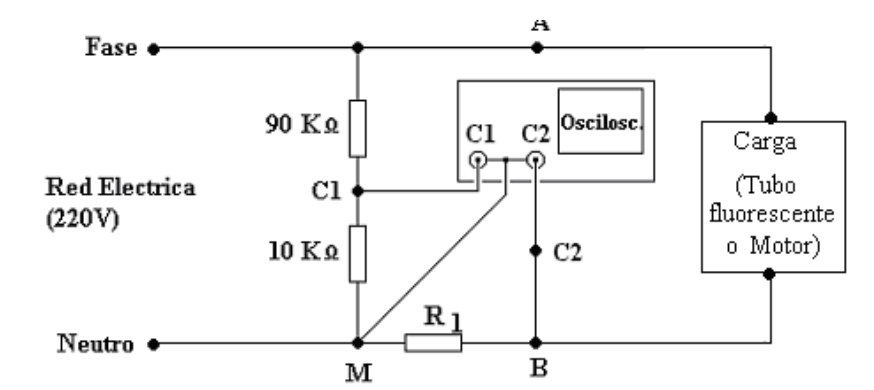
\includegraphics[width=0.5\textwidth]{images/esquema1.png}
    \caption{Conexiones realizadas}
    \label{fig:conexiones1}
\end{figure}

Ahora ajustaremos la sensibilidad del canal 1 y del canal 2, para luego ajustar la base de tiempo y así ver lo siguiente:

IMAGENES

Del modo X-Y (Segunda image), podremos obtener los valores de $sen(\phi)$ y $cos(\phi)$ mediante la siguiente formula:

\begin{equation*}
    cos(\phi) = \sqrt{1-(\frac{A}{B})^2}
\end{equation*}

\begin{equation*}
    sen(\phi) = \frac{A}{B}
\end{equation*}

Ahora con el multimetro para CA mediremos tension y corriente circulando por R1, y obtenemos los siguientes datos:

\begin{table}[H]
\resizebox{\columnwidth}{!}{%
\begin{tabular}{|lllcll|}
\hline
\multicolumn{1}{|l|}{} &
  \multicolumn{1}{c|}{Sens(V/div)} &
  \multicolumn{1}{c|}{Vpap} &
  \multicolumn{1}{c|}{\begin{tabular}[c]{@{}c@{}}Valores eficaces \\ (Tensión y corriente)\\ En Osciloscopio\end{tabular}} &
  \multicolumn{1}{c|}{\begin{tabular}[c]{@{}c@{}}Valores eficaces\\ Multímetro \\ True RMS\end{tabular}} &
  \multicolumn{1}{c|}{\begin{tabular}[c]{@{}c@{}}Incertidumbre\\ medición\\ multimetro\end{tabular}} \\ \hline
\multicolumn{1}{|l|}{Canal 1} & \multicolumn{1}{l|}{AA} & \multicolumn{1}{l|}{BB} & \multicolumn{1}{c|}{V =} & \multicolumn{1}{l|}{CC} & DD \\ \hline
\multicolumn{1}{|l|}{Canal 2} & \multicolumn{1}{l|}{EE} & \multicolumn{1}{l|}{FF} & \multicolumn{1}{c|}{I =} & \multicolumn{1}{l|}{GG} & HH \\ \hline
\multicolumn{6}{|c|}{\$Cos(\textbackslash{}phi) ; Sen(\textbackslash{}phi) ; Tan(\textbackslash{}phi)}                                      \\ \hline
\multicolumn{6}{|c|}{Potencia Activa: P =}                                                                                                  \\ \hline
\multicolumn{6}{|c|}{Potencia reactiva: Q = II ; Potencia Aparente: S = JJ}                                                                 \\ \hline
\end{tabular}%
}
\end{table}

\section{Desarrollo Experimental 2}

Ahora para corregir el factor de potencia, añadiremos un capacitor como elemento reactivo que compense el desfasaje entre tensión y corriente. Para ello antes debemos calcular el valor de la capacitancia necesaria para corregir el factor de potencia.

\begin{equation*}
    C = \frac{P \cdot tan(\phi)}{V^2 \cdot \omega}
\end{equation*}

Para este caso el valor de C es de AAAAA. Por lo que usaremos uno de FFFFF ya que tenemos que normalizar el valor.\\

Ahora conectaremos el capacitor entre los puntos A y B, paralelo a la carga y obtendremos lo siguiente:

IMAGEN

De estas mediciones obtenemos los siguientes datos:

\begin{equation*}
    V = AAAAAA
\end{equation*}
\begin{equation*}
    I = BBBBBB
\end{equation*}
\begin{equation*}
  S = CCCCCC
\end{equation*}

Como podemos ver estos datos son....

